%%%%%%%%%%%%%%%
%							TEST MODEL 
%%%%%%%%%%%%%%%

\subsection{Project Test Model}

\paragraph{}
This section outlines the test model that was created after the draft model stage, QUT data access and initial photovoltaic systems analysis. In order to create the test model of a ``real-world" Brisbane based commercial building to structure the analysis around, the QUT schematics and personal experience within Brisbane's built environment were integral. 

\subsubsection{Lighting Loads}

\paragraph{}
To calculate approximate lighting loads to be expected for a floor, level 6 of QUT P Block was marked up to count the number of luminaires installed. A full floor plan is shown in Appendix \ref{appendix:qut_lvl6_markup} but an image export is below in Figure \ref{fig:qut-lvl6-lighting-markup}.      

\begin{figure}[H]
	\hfill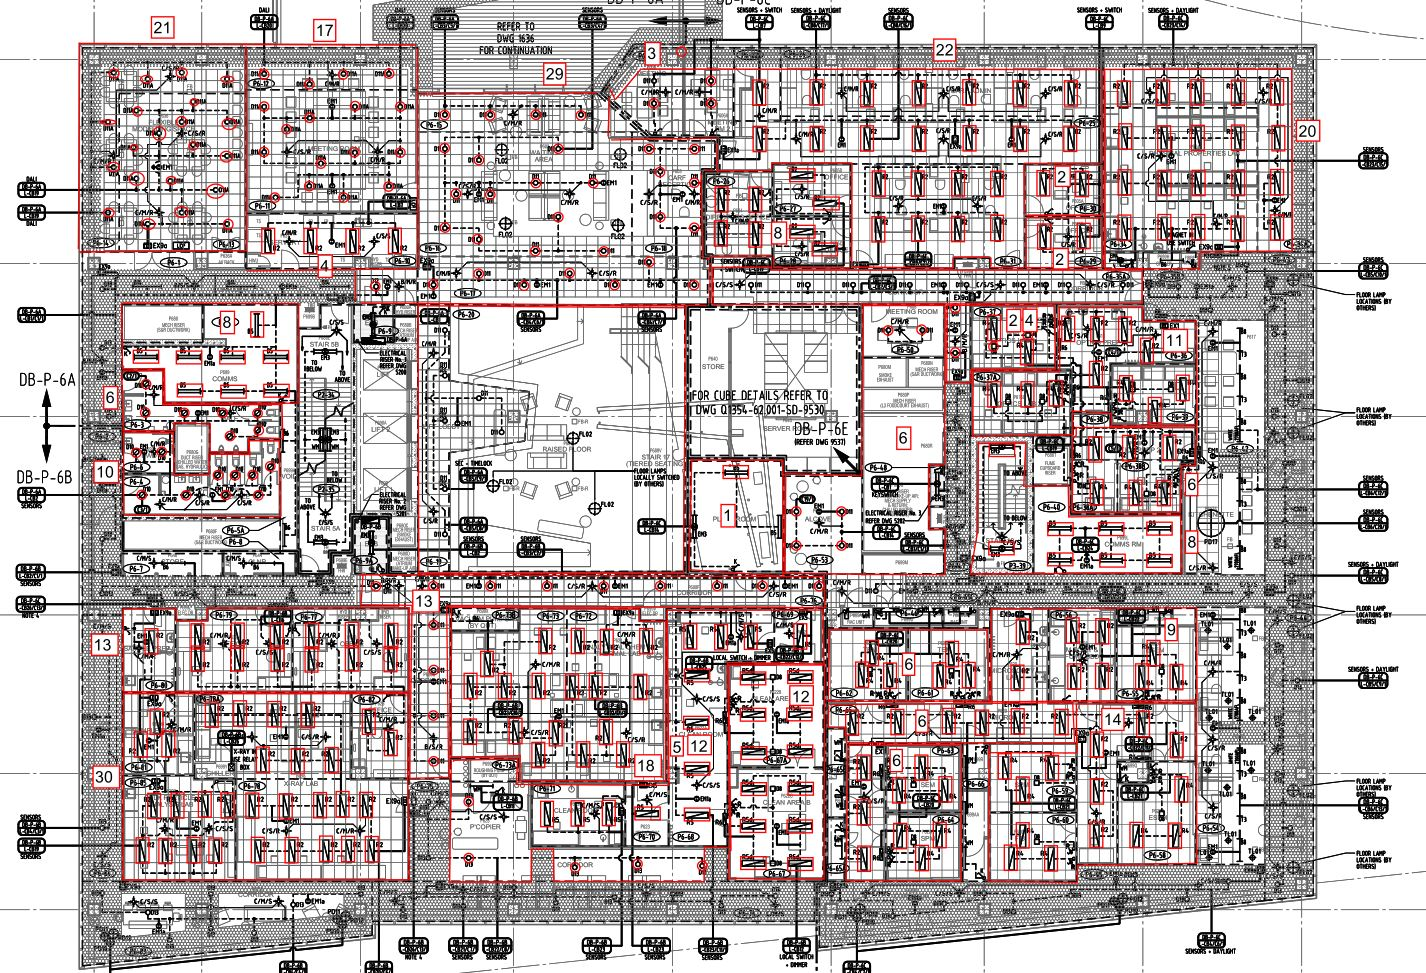
\includegraphics[width = 150mm]{images/project-model/qut-lvl6-lighting-markup}\hspace*{\fill}
	\caption{QUT: P Block Level 6 Lighting Markup} 
	\label{fig:qut-lvl6-lighting-markup}
\end{figure}

\paragraph{}
Table \ref{table:QUTlvl6-count} below outlines the counts from the markup. 

\begin{table}[!ht]
	\centering
	\renewcommand{\arraystretch}{2}
	\begin{tabular}{|c|c|c|c|c|}
		\hline
		\textbf{Fitting} & \textbf{Wattage (W)} & \textbf{Voltage (V)} & \textbf{Count} & \textbf{Demand (A)} \\ \hline
		LED Downlight & 36.0 & 24.0 & 110.0 & 165.0 \\ \hline
		LED Barlight & 56.0 & 24.0 & 224.0 & 522.7 \\ \hline
	\end{tabular}

	\caption{QUT: P Block Level 6 Lighting Count and Calculations}
	\label{table:QUTlvl6-count}
\end{table} 